%%%%%%%%%%%%%%%%%%%%%%%%%%%%%%%%%%%%%%%%%%%%%%%%%%%%%%%%%%%%%%%%%%%%%%%%%%%%%%%%
% --------------------------------------------------- ADD APPENDIX (IN CASE) ---
%%%%%%%%%%%%%%%%%%%%%%%%%%%%%%%%%%%%%%%%%%%%%%%%%%%%%%%%%%%%%%%%%%%%%%%%%%%%%%%%
\appendix

\chapter{Determining the resolution of the detector types}
\label{sec:ResDetermination}


A calibration spectrum of different kind of detectors used in \gerda\ has been constructed using different gamma sources at various energies (see figure \ref{fig:Aufloesung}).
In it two resolution functions were determined (see equation \ref{equ:BEGeCal} and \ref{equ:COAXCal}).
With these the full width at half maximum (FWHM) of a gamma lines in the respective detector types can be determined depending only on the energy of the gamma.
The FWHM corresponds to the resolution of the detectors.
It is therefor possible to determine the resolution of the detectors at the 514 keV line to $\Delta E_{\mathrm{BEGe}}] =2.26706\unit{keV}$ for the BEGe and $\Delta E_{\mathrm{COAX}}] = 2.72196\unit{keV}$ for the COAX.

\begin{figure}[t!]
	\centering
	\ifmakefigures%
	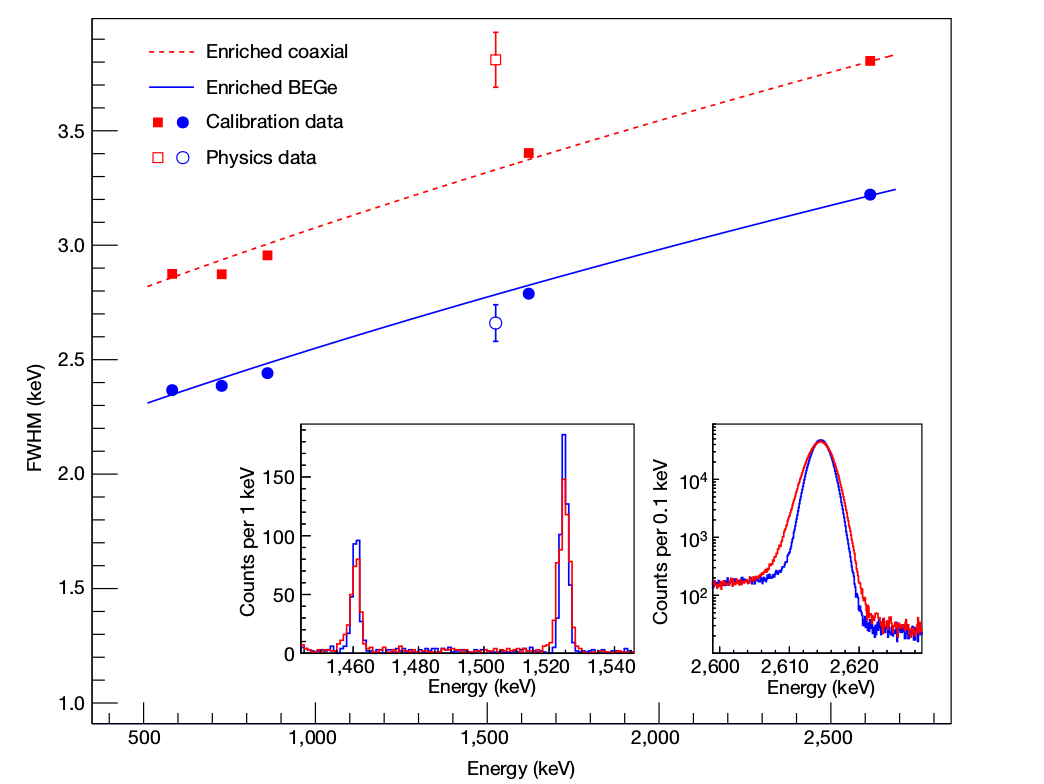
\includegraphics[width=80mm]{./Bilder/Aufloesung.png}
	\fi%
	\caption{
		The full width at half maximum (FWHM) of a investigated gamma lines in the respective detectors as a function of the energy of the investigated gamma.
		This value corresponds to the average resolution of the detectors at the respective energies.
		Taken from \cite{ahlswede_update_2013}.
	}
	\label{fig:Aufloesung}
\end{figure}

\begin{equation}
\Delta E_{BEGe}(x[keV]) = 2.35482 \times \sqrt{0.7065+0.0004286x}
\label{equ:BEGeCal}
\end{equation}

\begin{equation}
\Delta E_{COAX}(x[keV]) = 2.35482 \times \sqrt{1.01314+0.0006284x}
\label{COAXCal}
\end{equation}
\\

For the fit process it is also of interest to know the value of the expected variance $\sigma$ of the Gaussian peak functions.
With the FWHM this can easily be calculated by applying function \ref{equ:sigma}.

\begin{equation}
\sigma (\Delta E) = \frac{\Delta E}{2\sqrt{2\ln2}}
\label{equ:sigma}
\end{equation}

By applying this function one results in $\sigma_{BEGe} = 0.96273\unit{keV}$ and $\sigma_{COAX} = 1.15591\unit{keV}$ at an energy of 514 keV.



% \section{}
% \label{}
